
%\fitter\ is a unique QCD fit platform that provides many options to the user to perform a quantitative assessment of impact level for a new data or new theoretical prediction. The quest on nailing down the uncertainties on PDFs have lead, on one hand, to highly precise measurements that are in need of careful handling of all provided sources of uncertainties, and on the other hand to numerous software packages that provide higher order calculations in QCD to match the precision of data.



Nowadays, there are considerable number of choices available when performing a QCD fit analysis which require a careful investigation (i.e. input parametrisation form, threshold values for heavy quarks, various theory prescriptions, method of minimisation, interpretation of uncertaintes and so on).
%
 It is desirable to be able to discriminate or quantify the effect of chosen ansatz,  ideally within a framework that provides such cross checks and 
\fitter\ is optimaly designed for such tests.
%
The methodology employed by \fitter\  relies on a flexible and modular
framework that allows for independent integration of the state-of-the-art techniques, either related to the inclusion of a new theoretical calculation, or to a new approaches to treat uncertainties. 
%

In this section we briefly describe the available options in \fitter\ ranging from the functional form used to parametrise PDFs, presenting various representations of $\chi^2$ function, to different methods to assess the experimental uncertainties on extracted PDFs.

%list various types of functional forms used to parametrise PDFs, different definitions for  $\chi^2$ evaluation in extracting the PDF parameters which account for correlated and uncorrelated sources of experimental (or theoretical) uncertainties available in \fitter\. 
In addition, the reweighting method - an alternative approach to a complete QCD fit, available in the \fitter\ is also described in this section. It can provide for an estimate of an impact of new data, as advocated 
alreay by the NNPDF collaboration \cite{Ball:2011gg,Ball:2010gb}.
The method has been extended to work not only on the replica method, 
but also on the eigenvectors (as introduced by MSTW group \cite{Watt:2012tq}).

An important factor for a fesible QCD fit which is performed iteratively through the $\chi^2$ minimisation process,  represents the performance in terms of how long a calculation takes for each given data point.
In \fitter\ this is achieved by optimising the time of calculations relyng on innovative techniques such as cache option, fast evolution kernels, grid techniques making the platform a practical engine for iterative usage.


\subsection{Functional Forms for PDF parametrisation}
The PDFs are parametrised at the starting scale bellow the charm mass threshold, chosen by the user. Various functional forms can be tested using desired number of free parameters to be extracted through the fit:
\begin{description}
\item \bf {Standard Polynomials:} \rm
The term standard is understood to refer to a simple polynomial 
that interpolates between the low and high $x$ regions:
\begin{equation}
 xf(x) = A x^{B} (1-x)^{C} P_i(x),
\label{eqn:pdf_std}
\end{equation}
Standard forms are commonly used by PDF groups.
The parametrised PDFs at HERA are the valence distributions
 $xu_v$ and  $xd_v$,  the gluon distribution $xg$, and the $u$-type and $d$-type sea 
$x\bar{U}$, $x\bar{D}$, where $x\bar{U} = x\bar{u}$, 
$x\bar{D} = x\bar{d} +x\bar{s}$. 
The $P_i(x)$ for the HERAPDF style takes the simple form of $(1 + D x + E x^2)$ with additional constraints due to flavour decomposition insensitivity for $q\bar{s}$ fromother light sea quark contributions. 
For the CTEQ style, $P_i(x)$ takes te form of $e^{a_3x} (1 + e^{a_4} x + e^{a_5} x^2)$.


\item \bf {Log-Normal Distributions:} \rm
A bi-log-normal distribution to parametrise the $x$ dependence of the PDFs is available in \fitter\ .
%parton distribution function of the proton.
This parametrisation is motivated by  multiparticle statistics.
The following functional form can be used:
%\begin{center}
\begin{equation}
xf(x)=x^{p-b\log(x)}(1-x)^{q-\log(1-x)}.
\end{equation}
%\end{center}
This function can be regarded as a generalisation of standard functional form described above. In order to satisfy the QCD sum rules this parametric form requires numerical integration.

\item \bf {Chebyshev Polynomials:} \rm

A flexible Chebyshev polynomial based parametrisation can be used for the gluon and sea densities. The polynomials
use $\log x$ as an argument to emphasize the low $x$ behavior. 
The parametrisation is valid for $x>x_{min} = 1.7\times 10^{-5}$. The PDFs are multiplied
by $1-x$ to ensure that they vanish as $x\to 1$. The resulting parametric form is 
\begin{eqnarray}
x g(x) &=& A_g \left(1-x\right) \sum_{i=0}^{N_g-1} A_{g_i} T_i \left(-\frac{\textstyle 2\log x - \log x_{min} } {\textstyle \log x_{min} } \right)\,, \label{eq:glu} \\
x S(x) &=& \left(1-x\right) \sum_{i=0}^{N_S-1} A_{S_i} T_i \left(-\frac{\textstyle 2\log x - \log x_{min} } {\textstyle \log x_{min} } \right)\,. \label{eq:sea} 
\end{eqnarray}
Here the sum over $i$ runs up to $N_{g,S}=15$ order Chebyshev polynomials of the first type $T_i$ for
the gluon, $g$, and sea-quark, $S$, density, respectively. 
The normalisation $A_g$ is given by the momentum sum rule.

The advantages of this parametrisation are that the momentum sum rule can be evaluated analytically 
and that for $N \ge 5$ the fit qulaity is already similar
to a standard Regge-inspired parametrisation with a similar number of parameters.

\item \bf{External PDFs:} \rm 
\fitter\ provides also possibility to access the  external PDF sets, which can then be used in constructing the theoretical predictions rather than the ones restricted only to the \fitter\ framework. This is possible via interface to LHAPDF which commonly provides access to the global PDF sets available at LO, NLO or NNLO evolved either locally through the \fitter\ or taken as provided by the LHAPDF grid. Figure \ref{fig:pdfs} is produced with the drawing tools available in \fitter and illustrates the PDFs accessed from LHAPDF. 
\end{description}

\begin{figure}[!ht]
   \centering
   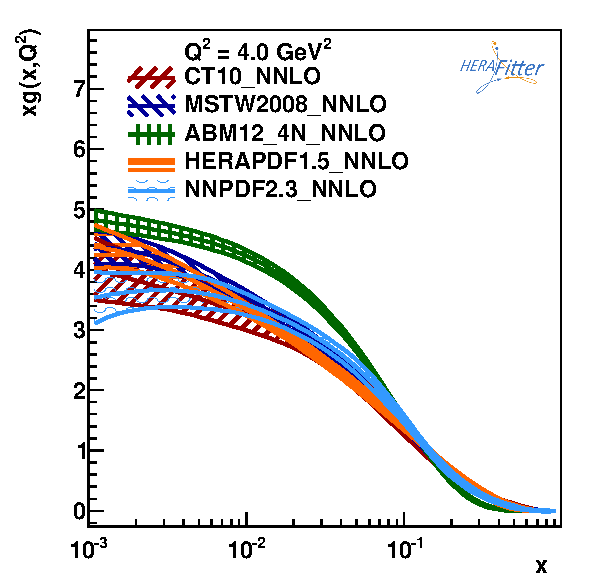
\includegraphics[width=8cm]{pdfs.pdf}
   \caption{Gluon density as extracted by various PDF groups at the scale of $Q^2=2$ GeV$^2$, plotted using the drawing tools from \fitter.} 
 \label{fig:pdfs}
\end{figure}

\subsection{Chisquare representation}


The PDF parameters are extracted from the $\chi^2$ minimization process. 
There are various forms to represent the $\chi^2$ function, i.e. covariance matrix or decomposed into nuisance parameters. In addition, there are various methods in dealing with the correlated systematic (or statistical) uncertainties. Here we summarise the options available in \fitter\ . 

\begin{description}
\item \bf {Covariance Matrix Representation:} \rm
For a data point  $\mu_i$ with a corresponding theory prediction $m_i$, the $\chi^2$ function for the case when experimental uncertainties are given in a covariance matrix over data bins $C_{i,j}$ can be expressed in the following form:

\begin{eqnarray}
\chi^2 (m)& = & \sum_{i,j}(m_i-\mu_i)C^{-1}_{ij}(m_j-\mu_j).
\end{eqnarray}
The $\chi^2$ function depends on the theory parameters $m^i$ 
(denoted as the vector $\boldsymbol{m}$).
The covariance matrix can be decomposed in statistical, uncorrelated and correlated systematic contributions: 
\begin{eqnarray}
C_{ij}& = & C^{stat}_{ij}+C^{uncor}_{ij}+C^{sys}_{ij}.
\end{eqnarray}

This representation can not single out the effect of a particular
source of systematic.

\item \bf{Nuisance Parameters Representation:} \rm


\begin{eqnarray} 
    \chi^2\left(\boldsymbol{m},\boldsymbol{b}\right) &= &  
 \sum_i \frac{\left[m^i - \sum_j \gamma^i_j m^i b_j  - {\mu^i} \right]^2}
{ \textstyle \delta^2_{i,{\rm stat}}\mu^i \left(m^i -  \sum_j \gamma^i_j m^i b_j\right)
  + \left(\delta_{i,{\rm uncor}}\,  m^i\right)^2} \nonumber \\
  &+& \sum_j b^2_j.
\label{eq:aven}
\end{eqnarray}
%
Here ${\mu^i}$ is the  measured central value  at a point $i$ 
with  relative statistical $\delta_{i,stat}$ 
and relative uncorrelated systematic uncertainty $\delta_{i,unc}$.
Further, 
%$\beta_j$ denotes a nuisance parameter for
% a correlated systematic error  source of type $j$ with an uncertainty while
$\gamma^i_j$ 
quantifies the sensitivity of the
measurement ${\mu^i}$ at the point $i$ to the systematic source $j$. 
The function $\chi^2$ depends in addition on
 the set of systematic uncertainties $b_j$ ($\boldsymbol{b}$).
This definition of the $\chi^2$ function takes into account that
systematic uncertainties are proportional to the central values 
(multiplicative errors), whereas the statistical errors scale 
with the square roots of the expected number of events. 
\item  \bf{Mixed Form:} \rm
It can happen that various parts of the systematic and statistical uncertainties are stored in different forms.  A user case can be envisaged when the correlated systematic experimental uncertainties are provided as nuisance parameters, but the statistical bin-to-bin correlation (non-negligible) given in forms of a covariance matrix. \fitter\ offers the possibility to include such information, when provided, as well as any other mixed form of treating statistical, uncorrelated and correlated systematic uncertainties. 
%In the case of off-diagonal statistical uncertainties, the $\chi^2$ function
is
%\begin{equation} 
%\begin{eqnarray} 
% \label{eq:chi2gen}
%    \chi^2(\boldsymbol{m},\boldsymbol{b})& = & \sum_{ij} 
%         \left ( m^i - \sum_l \gamma^i_l(m^i)b_l - \mu^i \right)  C^{-1}_{{\rm stat.}~ij}(m^i,m^j) \nonumber \\  
%    && \left(  m^j - \sum_l \gamma^j_l(m^j)b_l - \mu^j \right) +  \sum_l b^2_l.
%\end{eqnarray}
%\end{equation}
%Here the scaling properties of the correlated systematic uncertainties 
%$\Gamma^i_j$ and
%of the covariance matrix $C_{{\rm stat.}~ij}$ are expressed as a dependence
%on $m_i$ and the dependence of $\delta_{\rm stat}$ on $b_j$ is ignored.
\end{description}


\subsection{Treatment of the Experimental Uncertainties}

\fitter\ provides three methods in assessing the experimental uncertainties on PDFs: Hessian, Offset, and Monte Carlo method, which are described below.
Figure \ref{fig:error} shows a visual illustration of these various techniques which can be applied and drawn with \fitter.
\begin{figure}[!ht]
   \centering
   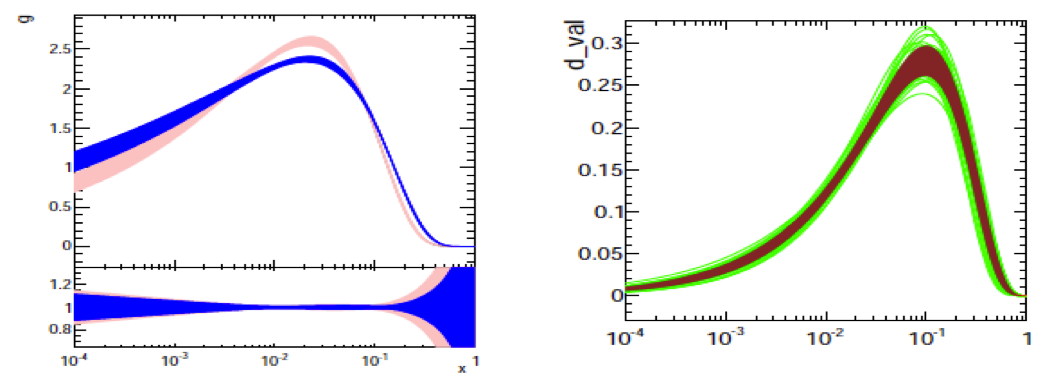
\includegraphics[width=8cm]{error.pdf}
   \caption{Differences in the experimental uncertainties on the gluon (left) and d-valence quark (right) densities extracted through various methods in \fitter: Hessian versus Monte Carlo.} 
 \label{fig:error}
\end{figure}
\begin{description}
\item \bf{Hessian method:} \rm
The technique developed by \cite{Pumplin:2001ct} presents an estimate of PDF uncertainties reflecting the experimental precision of used data in the QCD fit by examining the behaviour of $\chi^2$ in the neighborhood of the minimum. This is known as Hessian or error matrix method. The Hessian matrix is build by the second derivatives of $\chi^2$ at the minimum. The PDF eigenvectors are obtained through an iterative procedure used to diagonalise the Hessian matrix and rescale the eigenvectors to adapt the step sizes to their natural scale.

\item \bf{Offset  method:} \rm

There is another method to propagate the systematic experimental uncertainties from the measurements to PDFs \cite{Botje:2001fx}, which has the practical advantage that does not require the inversion of a large measurement covariance matrix.
%
It uses also the $\chi^2$ function for the central fit for which only
uncorrelated uncertainties are taken into account to get the best PDF parameters.
%
However, the goodness of fit can no longer be judged since correlated uncertainties are ignored. 
%
In the offset method, the systematic uncertainties on PDFs are estimated from fits where each systematic source is offset by its given one sigma shift to the central cross section values, after which the 
resulting deviation from the central PDF parameters are added in quadrature. 

In most cases, the uncertainties estimated through offset method are larger than these from the Hessian method, as offset method is not so efficient.

\item \bf{Monte Carlo method:} \rm
The PDF uncertainties can be estimated using a Monte Carlo technique \cite{Giele:1998gw, mcmethod2}.
The method consists in preparing replicas of data sets by allowing the central values of the cross sections to 
fluctuate within their systematic and statistical uncertainties taking into account all point-to-point correlations.
The preparation of the data is repeated for a large $N$ ($>100$ times) and for each of these replicas a NLO QCD fit is performed to 
extract the PDF set. The PDF central values and uncertainties are estimated using the mean values and RMS 
over the replicas. 
\end{description}


\subsection{Treatment of the Theoretical Input Parameters}

The results of a QCD fit depends not only on the input data but also on the 
input theoretical ansatz, which is also uncertain. Nowadays, the modern PDFs 
try to address the impact of this ansatz on the resulting PDFs by assessing an 
uncertainty on the choice of the initial parameter, such as mass of charm $m_c$, mass of the bottom quarks $m_b$. Another important input is the choice of the functional form for the PDFs at the starting scale. 
For this, HERAFitter provides a series of choices ranging from simple functional forms to more complex forms such as Chebyshev Polynomials with larger flexibility. Larger flexibility usually requires some regularisation methods in order for the results to be physical.




\subsection{Performance Optimisation}

The above mentioned features make \fitter a powerful project that encapsulates the state of the art developments from struggles on reaching atmost 
experimental precision to the most up-to-date theory developments. 

The performance of the \fitter  code is greatly improved with several special build-in options
including the $k-factor$ techniques (described in section~\ref{dissection}), the grid techniques for the fast calculational of cross 
sections of particular processes for arbitrary sets of PDFs (sections~\ref{dysection} and \ref{jetsection}) 
and usage of the openMP (Open Multi-Processing) interface which allows
parallel applications of some of the heavy flavour scheme theory prediction calculations in DIS. 



